\section{Heurística constructiva golosa}
\subsection{Introduccion}
Dado que la complejidad del algoritmo exacto resulta prohibitiva en la práctica, podemos aplicar heurísticas que resuelvan el problema en tiempo polinomial, a cuestas de la calidad final de la solución.

Las heurísticas tienen un factor importante de intuición sobre por qué podrían llegar a funcionar mejor o peor y no justificación formal. Debido a esto es difícil decidir qué criterio utilizar puesto que siempre es posible encontrar instancias para las cuales la heurística sea mala.

Nosotros decidimos encarar el criterio de una manera simple y segura, agregar nodos a la clique que nos aumenten la frontera de nuestra clique actual, hasta que no nos queden más aristas por agregar a la clique que nos aumenten la frontera.

\subsection{Desarrollo}
A la hora de aplicar esta heurística sobre nuestro problema, debimos poner el foco sobre donde queríamos realizar la construcción golosa. Rápidamente, y considerando que al utilizar la idea greedy debemos siempre tomar la decisión que mejora nuestra solución de manera óptima a corto plazo (es decir, que dada una clique de tamaño $n$, se obtiene la mejor solución de tamaño $(n+1)$ que contiene a la clique anterior), notamos que la forma acertada de aplicar esta heurística sería, en cada paso, agregar el nodo de mayor grado que genere una clique y mejore la frontera. Es decir que en el primer paso tomaremos siempre al nodo de mayor grado (puesto que esta es la clique de máxima frontera de tamaño 1) y en cada paso le agregaremos el nodo de mayor grado que sea adyacente a toda la clique y que mejore la frontera.

Es importante, antes de seguir, marcar algunas cosas importantes sobre nuestra solución. Para empezar, consideremos que cada vez que agregamos un nodo nuevo a la clique, debemos sumar el grado del nuevo nodo y restar dos veces el tamaño de la subclique (una vez para descontar las aristas que van del nuevo nodo a la clique, y otra para descontar las aristas que iban de cada nodo de la clique al nuevo nodo). Simplificando, tenemos que realizar el siguiente cálculo:

\begin{center}
Para $V_i$ vértice que se agrega a subclique
$Frontera(Clique) = Frontera(Subclique) + d(V_i) - tam(subclique)$ $\times$ $2$
\end{center}

Como vemos, la única variable que cambia cada vez que agregamos un nodo a la clique es el grado del mismo. Por lo tanto, sabemos que si agregar el nodo de mayor grado posible implica empeorar la frontera, entonces todos los nodos de menor grado a él también la empeoraran (lo cual, visto de otra forma, significa también que agregar ese nodo implica tomar la mejor decisión a corto plazo).

Por lo tanto, sabemos que estamos tomando siempre la mejor decisión rápida. Ahora bien, es importante marcar que, llegado el punto en el cual no conseguimos una manera de agrandar la clique mejorando la frontera, la mejor decisión es detenerse. Esto implica no solo que no podemos dar el próximo paso sin achicar la frontera, sino que a partir de este punto no se podrá mejorar la frontera en ningún paso. Esto es fácil de ver si consideramos lo que vimos antes: si el nodo de mayor grado posible empeora la frontera, todos los de grado menor a él también lo hacen. Supongamos que, efectivamente decidimos agregar un nodo $j$ a la clique, de manera que nuestra frontera disminuya, pero luego encontramos un nodo $i$ que podemos agregar a la clique de forma que la frontera crezca. Esto implicará lo siguiente:

\begin{center}
Para $C$ clique original, $C_i$ clique con nodo i, $C_{ij}$ clique con nodos i y j.
$$Frontera(C_i) = Frontera(C) + d(i) - tamano(C) \times 2$$
$$Frontera(C_{ij}) = Frontera(C_i) + d(j) - (tamano(C) + 1) \times 2$$

Vimos que $Frontera(C_{ij})$ $>$ $Frontera(C_i)$, lo cual implica $d(j) > (tamano(C) + 1) \times 2)$, es decir, $d(j) > tamano(C) \times 2$

Pero $Frontera(C_i)$ $<$ $Frontera(C)$, lo cual implica $d(i) < tamano(C) \times 2$

Por lo tanto, tenemos $d(j) > tamano(C) \times 2 > d(i)$, es decir, $d(j) > d(i)$. Pero entonces, eso implica que al agregar el nodo $i$ no agregamos el de mayor grado, puesto que $j$ es adyacente a todos los nodos de $C$ y es de mayor grado que $i$. Absurdo.
\end{center}

De este modo, tenemos una heurística constructiva golosa válida, que toma siempre la mejor decisión posible relacionada al próximo paso y se detiene cuando ya no hay forma de agrandar su frontera agregando nodos a la clique. Considerando entonces este desarrollo, obtenemos el siguiente algoritmo:

\begin{algorithm}[H]
	\NoCaptionOfAlgo
	\caption{\algoritmo{constructivaGolosa}{\In{listaAdyacencia}{lista}}{clique}}

    mayor $\leftarrow$ nodoDeMayorGrado(lista)

    agregarNodoAClique(res, mayor])

    nodosAdyacentes $\leftarrow$ adyacentes(lista, mayor)

    ordenarPorGrado(nodosAdyacentes)

    \For{$i \leftarrow 0$ \KwTo nodosAdyacentes.largo}{
		\If{esAdyacenteATodos(nodosAdyacentes[i], res, listaAdyacencia) $\land$ \\ aumentaLaFrontera(nodosAdyacentes[i], res, listaAdyacencia)}{
			agregarNodoAClique(res, nodosAdyacentes[i])

	}
}
\end{algorithm}

\subsection{Complejidad Temporal}

Esta implementación es bastante sencilla y solo utiliza unas pocas funciones. Veamos la complejidad temporal en peor caso de ellas para después ver la del algoritmo general.

\begin{itemize}
    \item \textbf{nodoDeMayorGrado}: Recorre los n nodos en la lista y se fija el largo de sus adyacentes en $O(1)$ por lo que la función es $O(n)$.

	\item \textbf{ordenarPorGrado}: Esta función utiliza por detrás el sort de la STD, y por ende su complejidad en peor caso es de $O(n*log(n))$. Como sabemos que no recorremos los $n$, sino $|maxAdyacente|$,  podríamos acotarlo por $O(|maxAdyacente|*log(|maxAdyacente|))$

    \item \textbf{esAdyacenteATodos}: Busca si hay un nodo en la clique que no sea adyacente a este nuevo nodo. Para eso, arma un arreglo de booleanos del tamaño del grafo ($O(n)$) y recorre los nodos adyacentes al nodo a insertar (pueden ser hasta $n-1$). Después, basta con recorrer los nodos de la clique y fijarse en el arreglo si son adyacentes o no. Siguiendo este procedimiento, el algoritmo tiene una complejidad temporal $O(n + |adyacentes| + |clique|)$. Es facil ver que $O(|maxClique|)$ $\subseteq$ $O(|maxAdyacentes|)$ , por lo que, si tomamos estas cotas, tendremos $O(n + |adyacentes| + |clique|)$ $\subseteq$ $O(n$ $+ |maxAdyacentes|$ $+ |maxClique|)$ $\subseteq$ $O(n + |maxAdyacentes| + |maxAdyacentes|)$. Veamos, entonces, que $|maxAdyacentes|$ esta acotado por $n - 1$ (puesto que un nodo puede llegar como máximo a todos los nodos del grafo que no son él) por lo que tenemos $O(|maxAdyacentes|)$ $\subseteq$ $O(n)$. Por ende, podemos afirmar $O(n + |maxAdyacentes| + |maxAdyacentes|)$ $\subseteq$ $O(n)$, y nuestra cota queda definida por el costo de armar el vector de booleanos.

    \item \textbf{aumentaLaFrontera}: Hace una simple aritmética entre la cantidad de nodos y la cantidad de adyacentes de la clique por lo que su complejidad es $O(1)$.

    \item \textbf{agregarNodoAClique}: Se encarga de actualizar la clique agregando atrás del vector de nodos en la clique el nodo a insertar en $O(1)$.

\end{itemize}

Ahora analicemos la complejidad de la heurística completa. Inicialmente buscamos el nodo de mayor grado y ordenamos sus adyacentes. Aquí, la operación más costosa es la de ordenar en un tiempo $O(|maxAdyacente|*log (|maxAdyacente|))$. Luego, tomamos el nodo de mayor grado y, para cada uno de sus nodos adyacentes, fijarnos si es posible agregarlo a la clique (es decir, si esAdyacenteATodos). Por lo tanto, para $|maxAdyacente|$ corremos un algoritmo de costo $O(n)$.

Sin embargo, así como vimos que $|maxAdyacente|$ $\leq$ (n - 1), es fácil ver que en un grafo de 40 nodos y 5 aristas, $|maxAdyacente|$ $\leq$ 5 (puesto que un nodo jamás tendrá 6 o más adyacencias, ya que eso implicaría tener 6 o más aristas en el grafo). Por ende, si extendemos esto a todos los grafos, vemos que $O(|maxAdyacente|)$ $\subseteq$ $O(min(n,m)$ , por lo que acabamos teniendo $O(min(n,m)$ $\times$ $O(n)$.

Por ende, al implementar la misma cota sobre ordenarPorGrado, tenemos las siguientes operaciones a considerar: se encuentra el nodo de mayor grado en $O(n)$, se ordena por grado en $O(min(n,m)$ $\times$ $log(min(n,m)))$, y se arma la clique en $O(min(n,m)$ $\times$ $n )$.  Entonces, nuestra cota temporal acaba siendo $O(n + min(n,m)$ $\times$ $log(min(n,m)) + min(n,m)$ $\times$ $n )$. Simplemente, vemos que $O(n)$ $\subseteq$ $O(min(n,m)$ $\times$ $n )$, y como $O(min(n,m))$ $\subseteq$ $O(n)$ (porque siempre $n$ será mayor o igual al mínimo entre $n$ y $m$) , tenemos que $O(min(n,m)$ $\times$ $log(min(n,m)))$ $\subseteq$ $O(min(n,m)$ $\times$ $n )$. Por lo tanto, nuestra cota acaba siendo $O(min(n,m)$ $\times$ $n )$.

\subsection{Casos Patológicos}

La heurística falla en el resultado máximo, cuando uno de los nodos de mayor grado que siguen formando la clique no pertenece a la del resultado esperado, si esto sucede, otros nodos de menor grado nos permiten conseguir en conjunto una mayor frontera.

\begin{SCfigure}[1][h]
\caption{En este caso podemos apreciar que si elegimos el nodo de máximo grado(5), esta va a ser nuestra frontera maximal. Pero en cambio la clique formada por los nodos de menor grado(4) en conjunto su frontera es mayor, obteniendo una frontera de 6.}
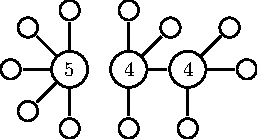
\includegraphics[width=0.5\textwidth]{img/patologic.pdf}
\end{SCfigure}

Podemos generar este tipo de grafos, teniendo una diferencia en el resultado máximo tan grande como queramos. Podemos definir una familia de instancias, que el nodo de mayor grado, digamos de grado k, tal que sus adyacentes son solo adyacentes a él (formando una frontera $k$), a este mismo grafo pertenece una clique de $\frac{k}{2}$ nodos y cada uno de estos además es adyacente a $\frac{k}{2}$ de grado 1. Los nodos de esta clique tienen grado $k - 1$ por lo que en la golosidad hubiésemos preferido el de grado $k$, pero la clique paralelamente construída tiene $\frac{k}{2}$ nodos con $\frac{k}{2}$ adyacentes no pertenecientes a la clique, por lo que la frontera es de $\frac{k}{2} \times \frac{k}{2} = \frac{k^2}{4}$.

Notemos que la diferencia de frontera es de $\frac{k^2}{4} - k$ por lo basta con tomar un $k$ mayor para que la diferencia sea tan grande como queramos, por lo que los grafos con esta particularidad la heurística arrojará malos resultados y estimaciones.

\subsection{Experimentación}

El desafío que nos encontramos al analizar la complejidad de nuestras heurísticas fue que las mismas dependían no solo de $n$ y $m$, sino de la relación entre las mismas. Para simplificar, decidimos obviar algunos casos promedio que resultaron dificultosos.

\noindent
\begin{minipage}{0.49\textwidth}
    \hfill
    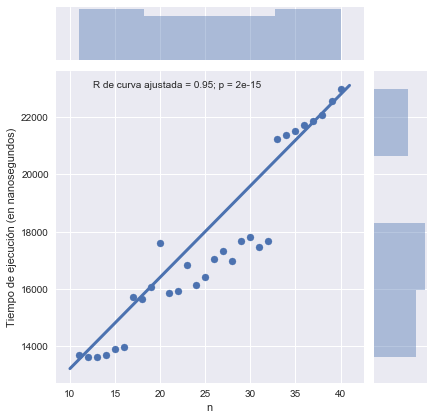
\includegraphics[scale=0.55]{img/greedy-n-low.png}

    \begin{center}
        Datos del gráfico

        \begin{tabular}{ | l l |}
            \hline
             & $m = 10$ \\ 
            Curva aproximada & $f(x) = 320 * x + 10000$ \\
            \hline
        \end{tabular}
    \end{center}
\end{minipage}
\hfill
\begin{minipage}{0.49\textwidth}
    \hfill
    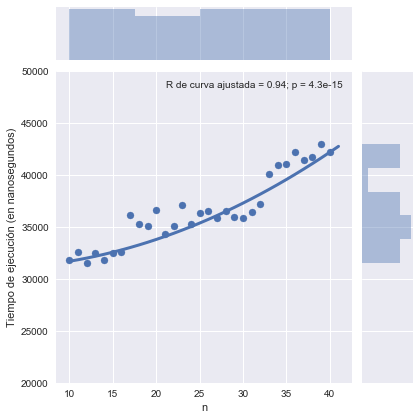
\includegraphics[scale=0.55]{img/greedy-n-hi.png}

    \begin{center}
        Datos del gráfico

        \begin{tabular}{ | l l |}
            \hline
             & $m = 40$ \\ 
            Curva aproximada & $f(x) = 7 * n^2 + 31000$ \\
            \hline
        \end{tabular}
    \end{center}
\end{minipage}

Como nuestra complejidad tiene un componente fijo $n$ y uno variable $min(n,m)$, decidimos

Nos resultó dificil medir el impacto del tamaño de la clique máxima, ya que la misma depende mucho de las aristas del grafo generado. Esto resultó en algunos resultados dispares. Sin embargo, podemos ver por el R de Pearson que nuestra aproximación  la correlación se aproxima a lineal.

\noindent
\begin{minipage}{0.55\textwidth}
    \hfill
    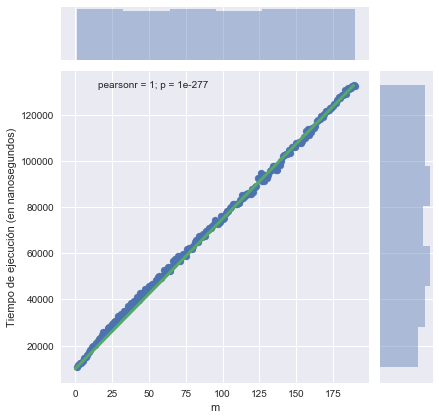
\includegraphics[scale=0.6]{img/greedy-m.png}
\end{minipage}
\hfill
\begin{minipage}{0.44\textwidth}
    \begin{center}
        Datos del gráfico

        \begin{tabular}{ | l l |}
            \hline
             & $n = 20$\\ 
            Curva aproximada & $f(x) = 580 * x + 10000$ \\
            \hline
        \end{tabular}
    \end{center}
\end{minipage}

Por otro lado, el impacto lineal de la cantidad de aristas fue más que evidente. Debido a la superposición de los puntos, la curva aproximada debió ser graficada en otro color.
